\chapter{{\bf Distributions of input variables for the global BDT}}
\label{sec:appendix1}
Comparison of the signal and background distributions of input variables used in the global BDT for 2011, 2012, 2015 and 2016 data taking conditions. Signal distributions are from simulated \bsmumu decays for each year that have passed the selection cuts in Table~\ref{tab:BDTpresel}. The background distributions are from \bbbarmumux decays in 2011, 2012, 2015 and 2016 data with $m_{\mu \mu} > 5447$ \mevcc and passing the selection cuts in Table~\ref{tab:BDTpresel}.
\begin{figure}
    \centering
    \begin{subfigure}[b]{0.48\textwidth}
        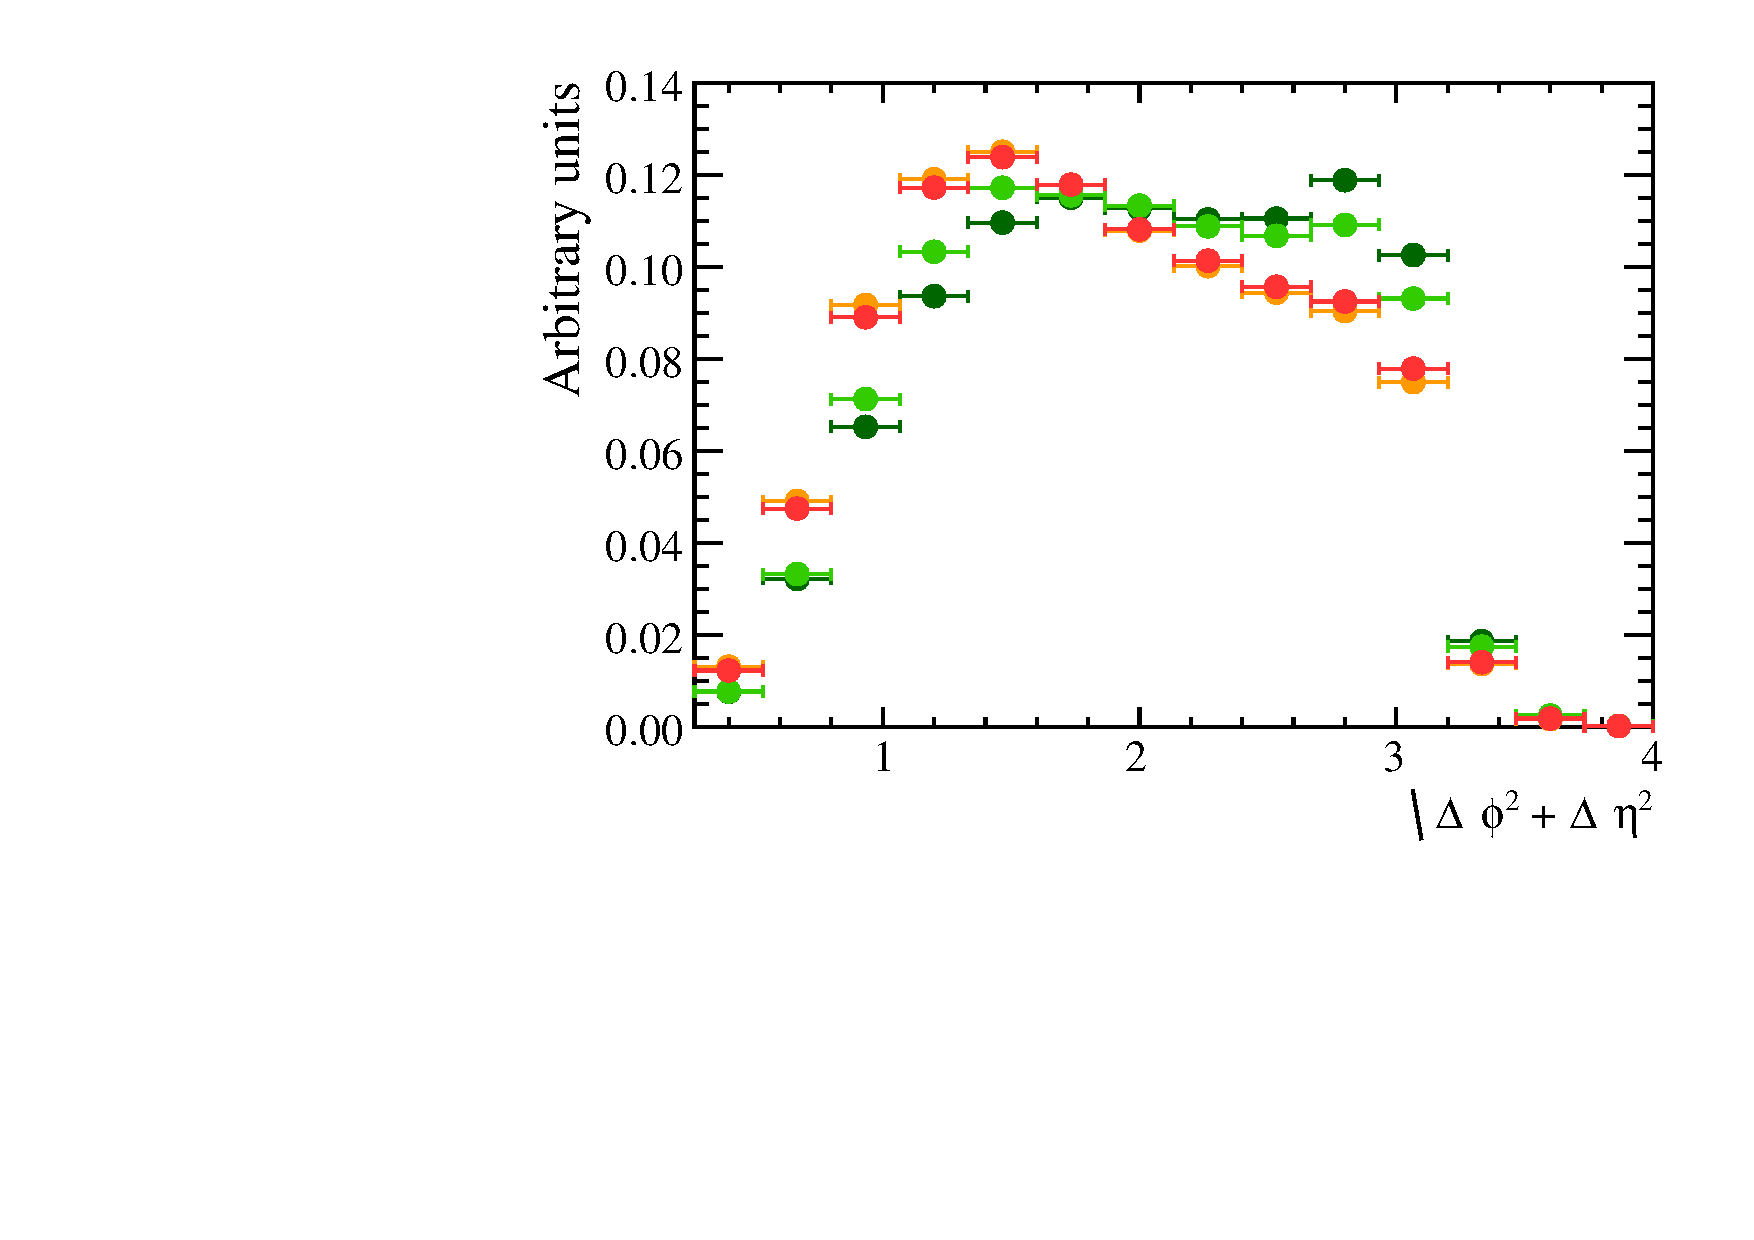
\includegraphics[width=\textwidth]{./Figs/Appendix1/signal_deltaR.pdf}
%        \caption{ }
%        \label{fig:BDTsig}
    \end{subfigure}
    ~ %add desired spacing between images, e. g. ~, \quad, \qquad, \hfill etc. 
      %(or a blank line to force the subfigure onto a new line)
    \begin{subfigure}[b]{0.48\textwidth}
       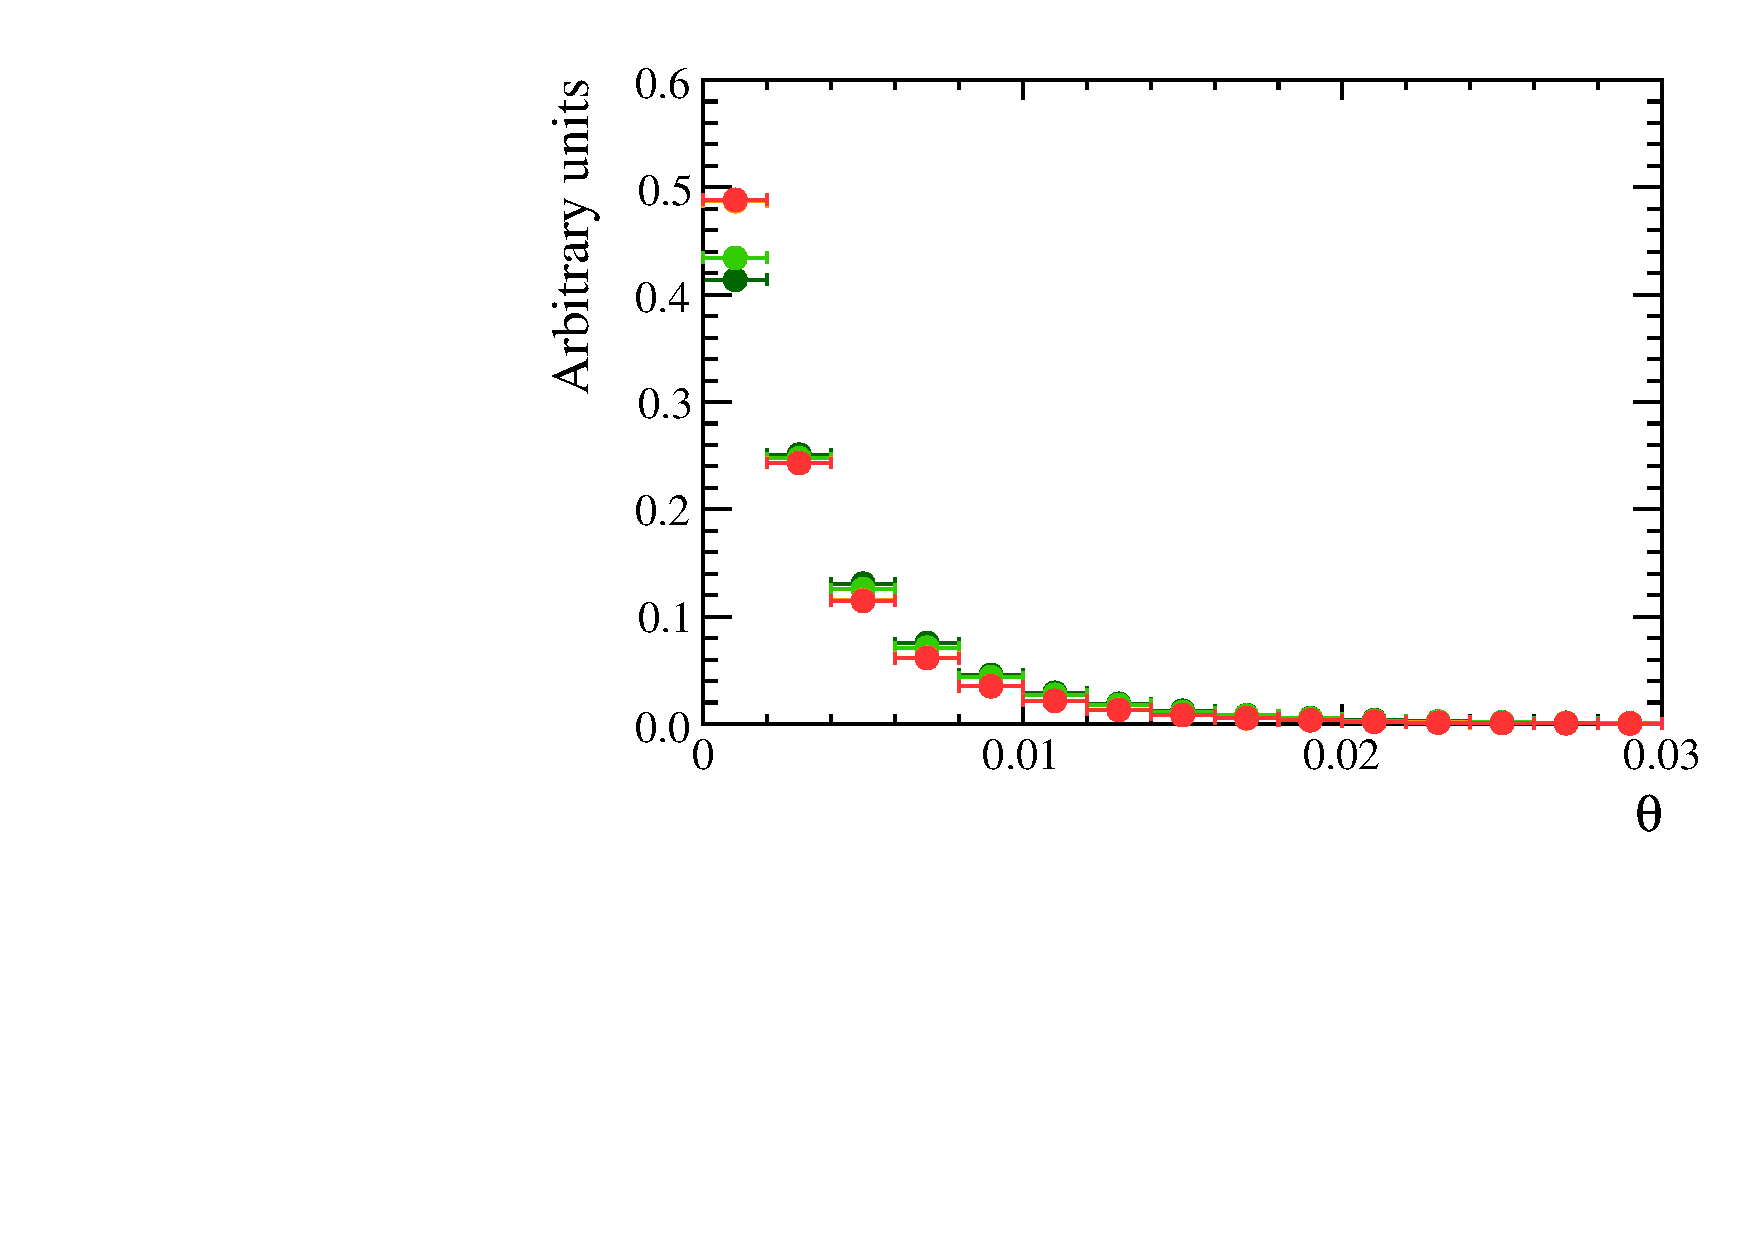
\includegraphics[width=\textwidth]{./Figs/Appendix1/signal_DIRA.pdf}
%        \caption{ }
%        \label{fig:BDTbkg}
    \end{subfigure}



 \begin{subfigure}[b]{0.48\textwidth}
        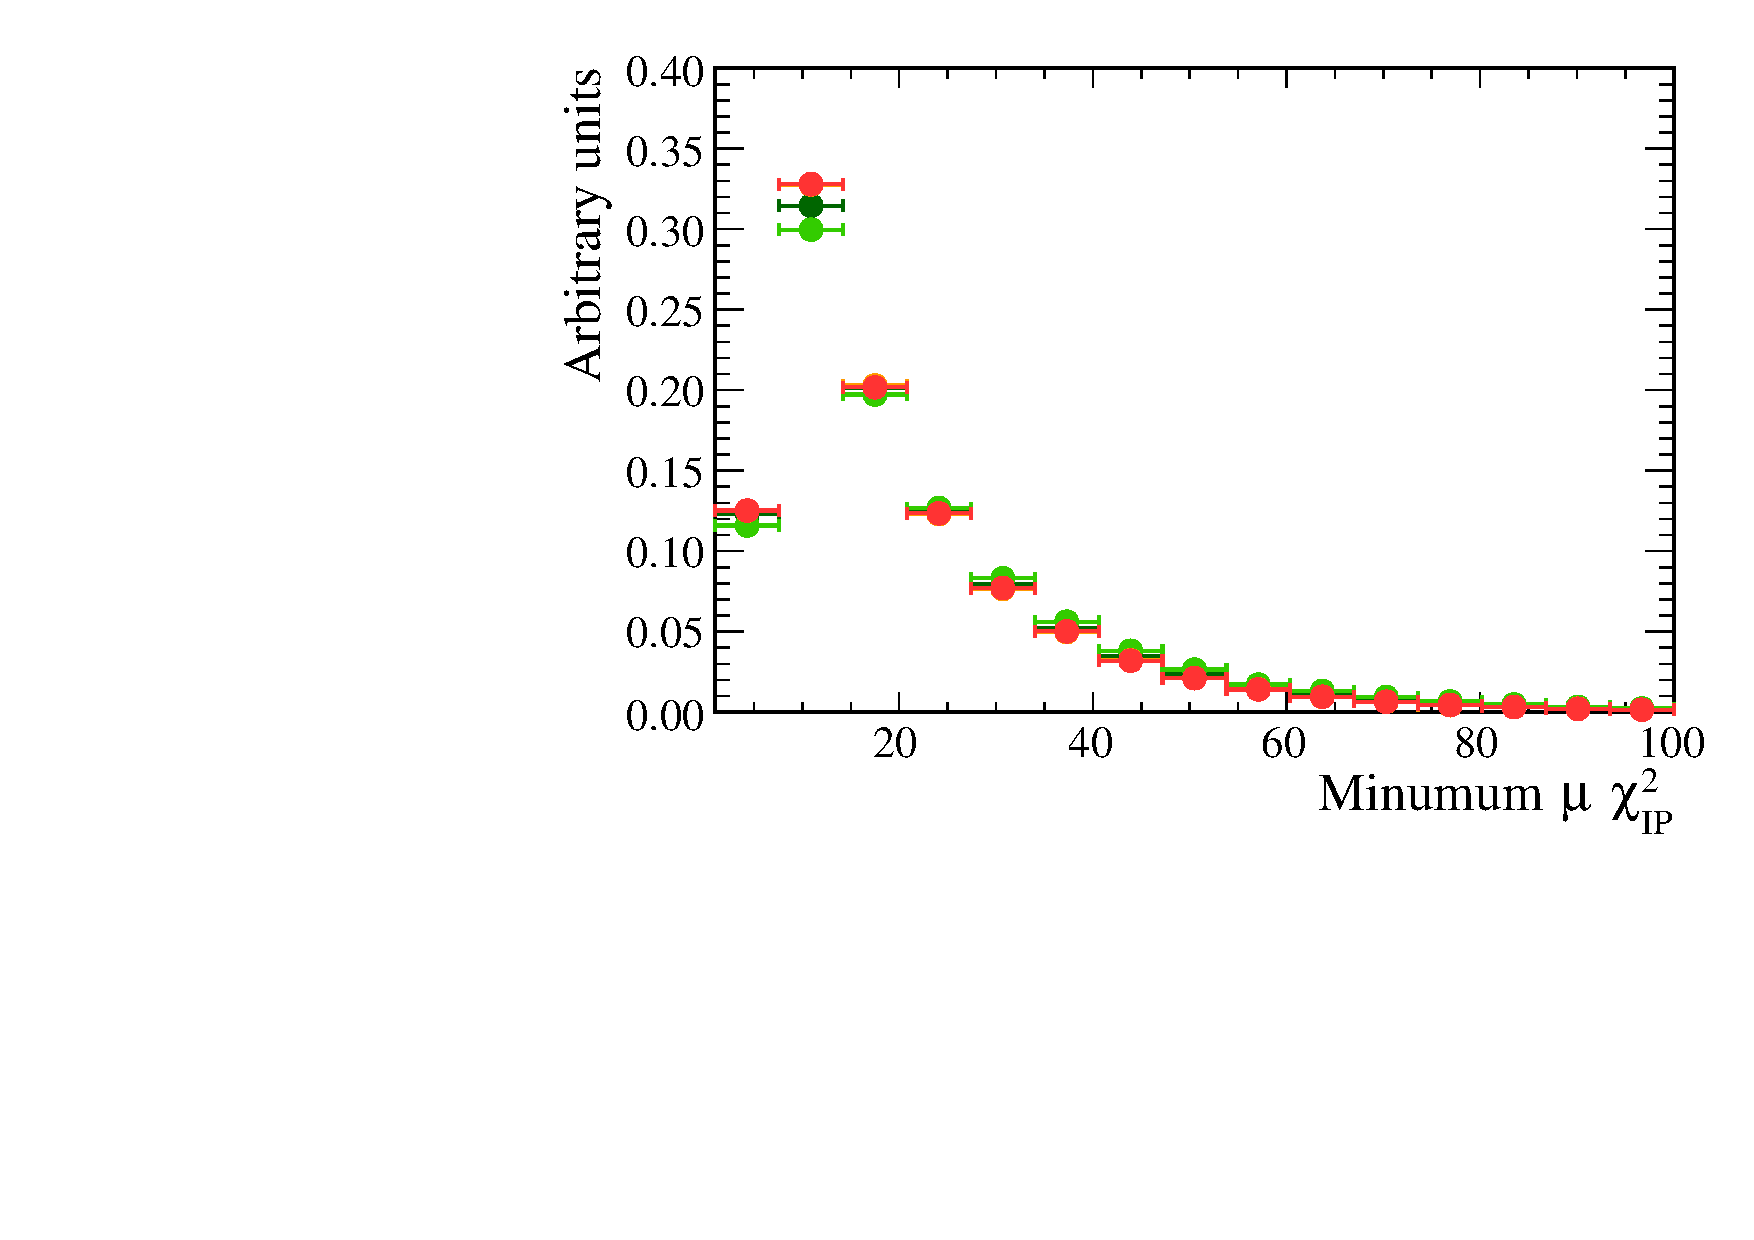
\includegraphics[width=\textwidth]{./Figs/Appendix1/signal_muIPS.pdf}
%        \caption{ }
%        \label{fig:BDTsig}
    \end{subfigure}
    ~ %add desired spacing between images, e. g. ~, \quad, \qquad, \hfill etc. 
      %(or a blank line to force the subfigure onto a new line)
    \begin{subfigure}[b]{0.48\textwidth}
       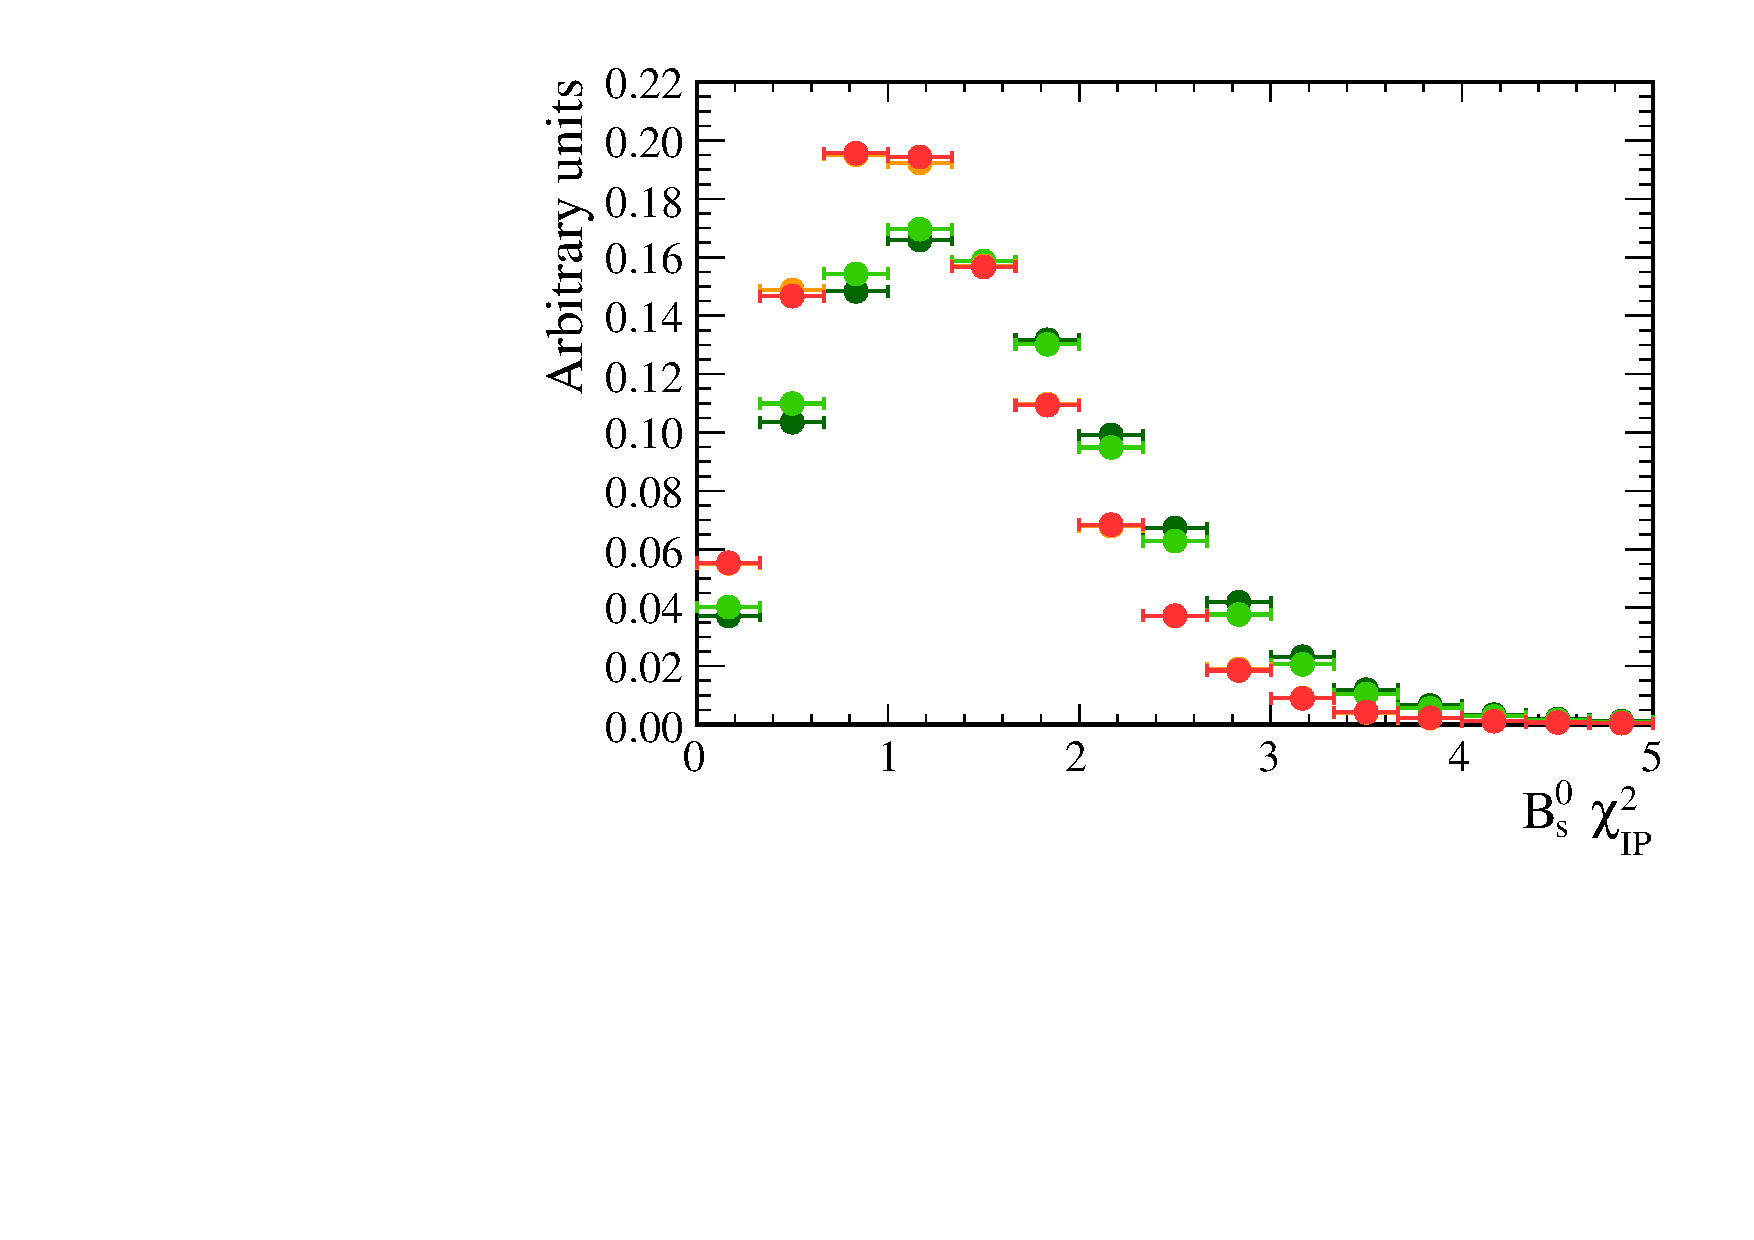
\includegraphics[width=\textwidth]{./Figs/Appendix1/signal_IPS.pdf}
%        \caption{ }
%        \label{fig:BDTbkg}
    \end{subfigure}





 \begin{subfigure}[b]{0.48\textwidth}
        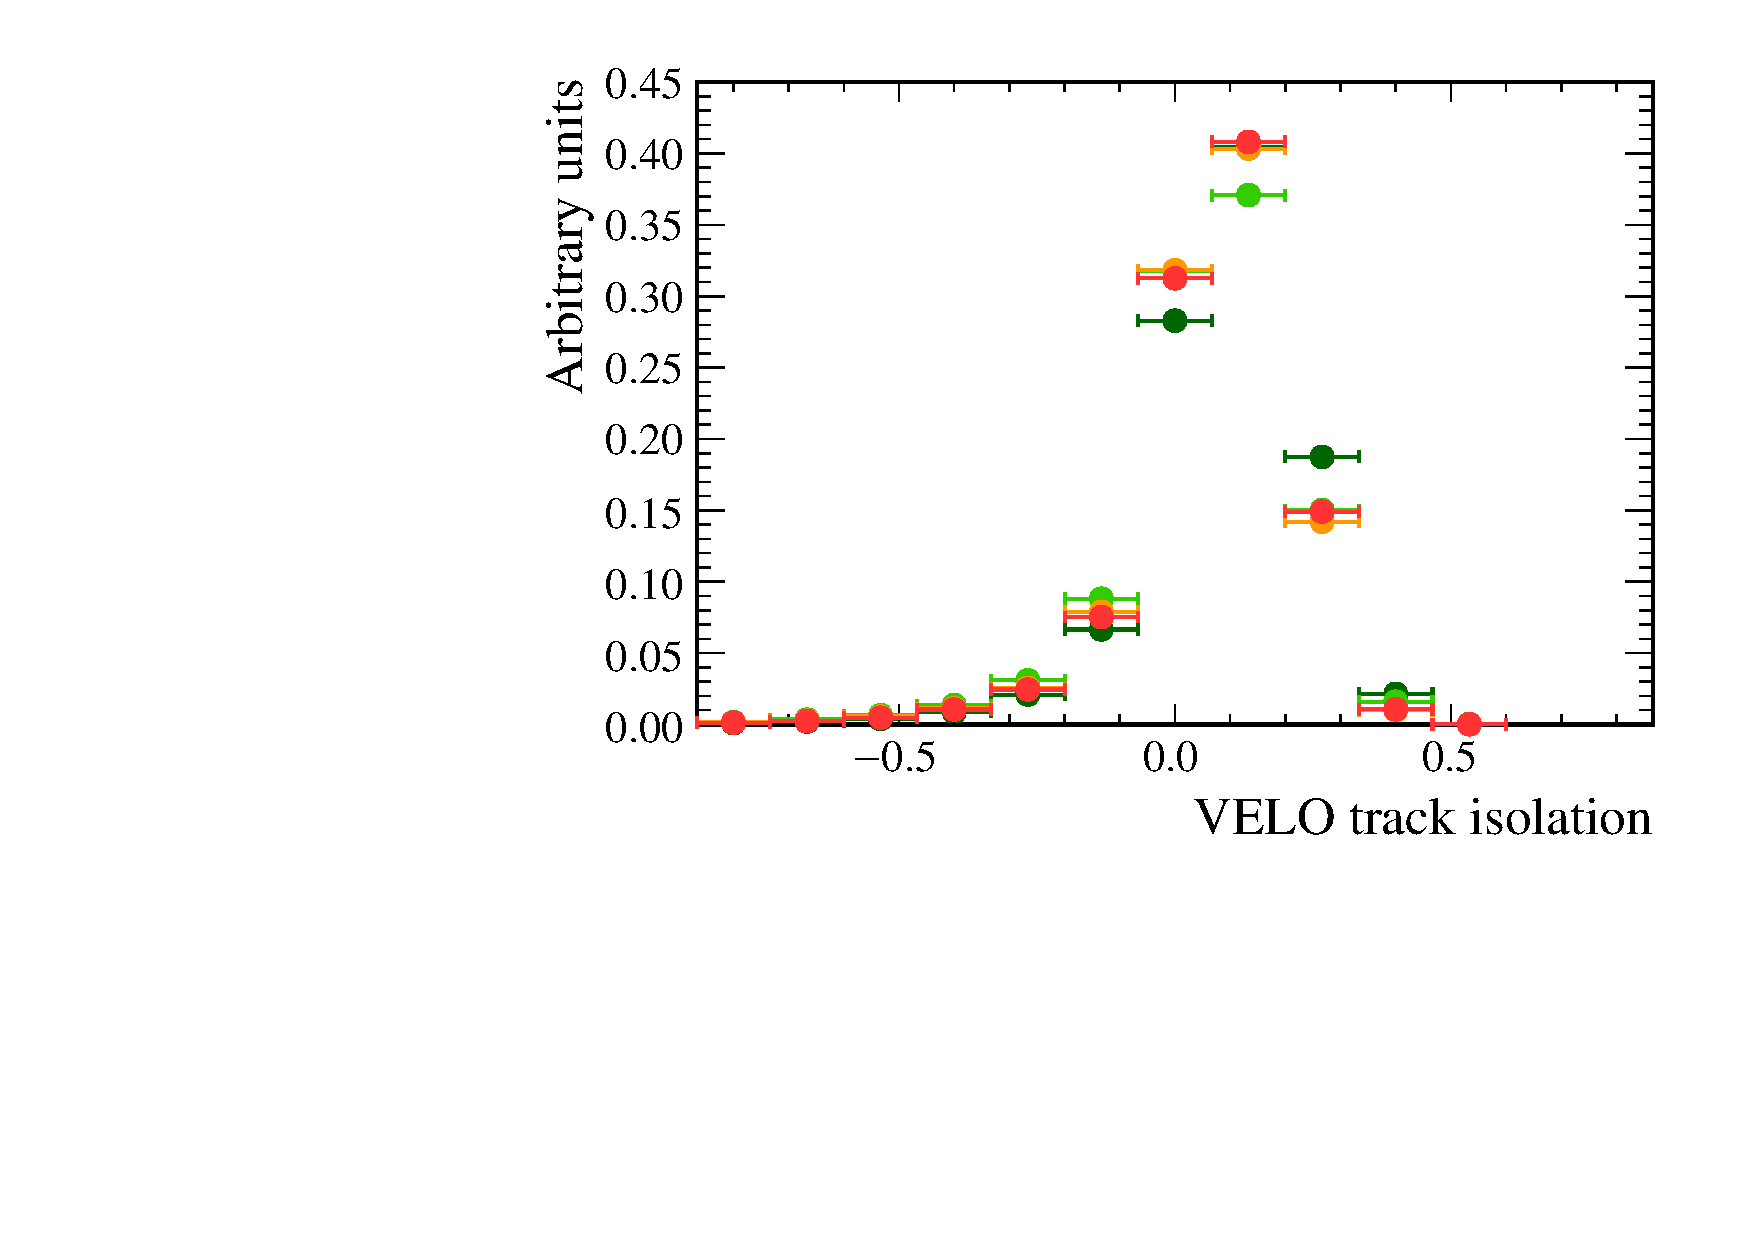
\includegraphics[width=\textwidth]{./Figs/Appendix1/signal_iso_velo.pdf}
 %       \caption{ }
 %       \label{fig:BDTsig}
    \end{subfigure}
    ~ %add desired spacing between images, e. g. ~, \quad, \qquad, \hfill etc. 
      %(or a blank line to force the subfigure onto a new line)
    \begin{subfigure}[b]{0.48\textwidth}
       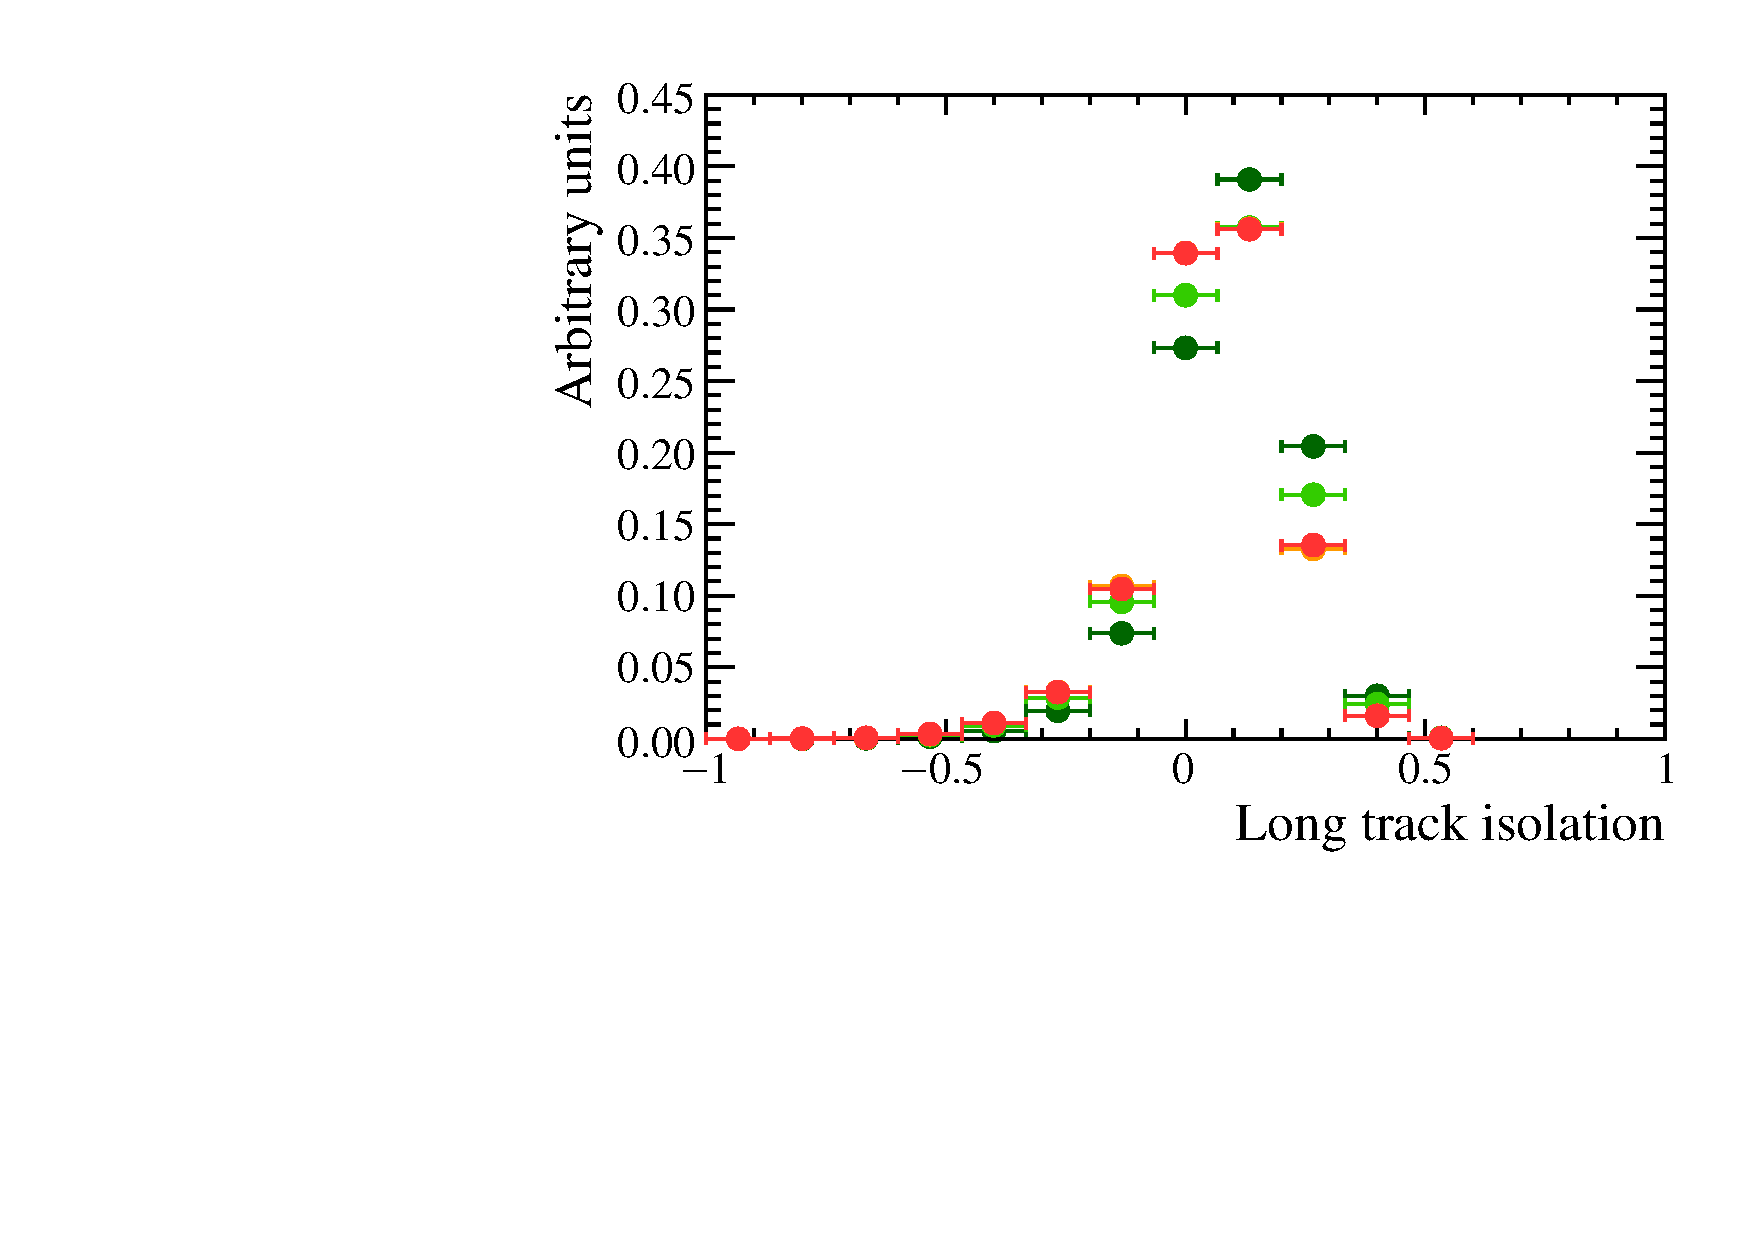
\includegraphics[width=\textwidth]{./Figs/Appendix1/signal_long_iso.pdf}
  %      \caption{ }
  %      \label{fig:BDTbkg}
    \end{subfigure}




 \begin{subfigure}[b]{0.48\textwidth}
        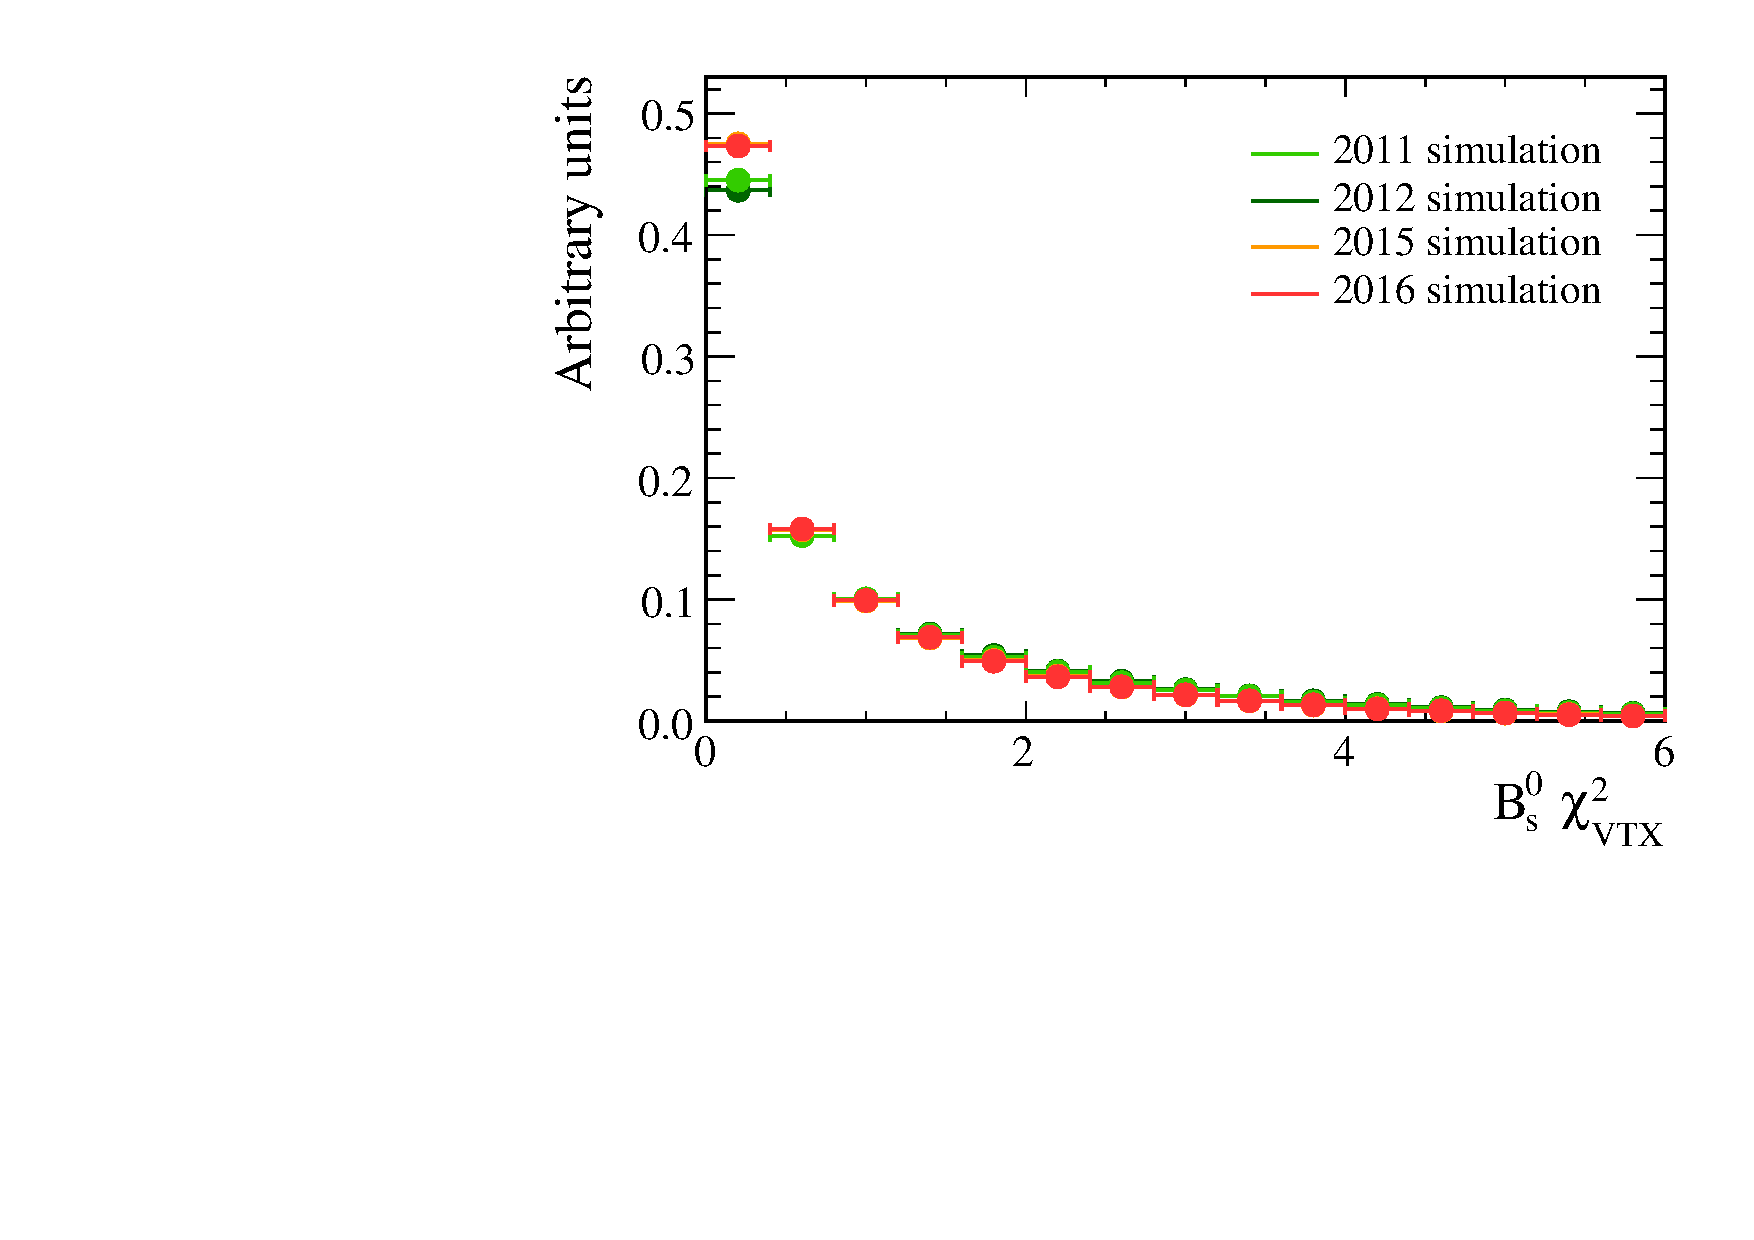
\includegraphics[width=\textwidth]{./Figs/Appendix1/signal_end_vertex.pdf}
   %     \caption{ }
   %     \label{fig:BDTsig}
    \end{subfigure}
    ~ %add desired spacing between images, e. g. ~, \quad, \qquad, \hfill etc. 
      %(or a blank line to force the subfigure onto a new line)
 



    \caption{Signal distributions for input variables for the global BDT for \bsmumu simulated decays in 2011, 2012, 2015 and 2016.}
    \label{fig:signalvars}
\end{figure}



\begin{figure}
    \centering
    \begin{subfigure}[b]{0.48\textwidth}
        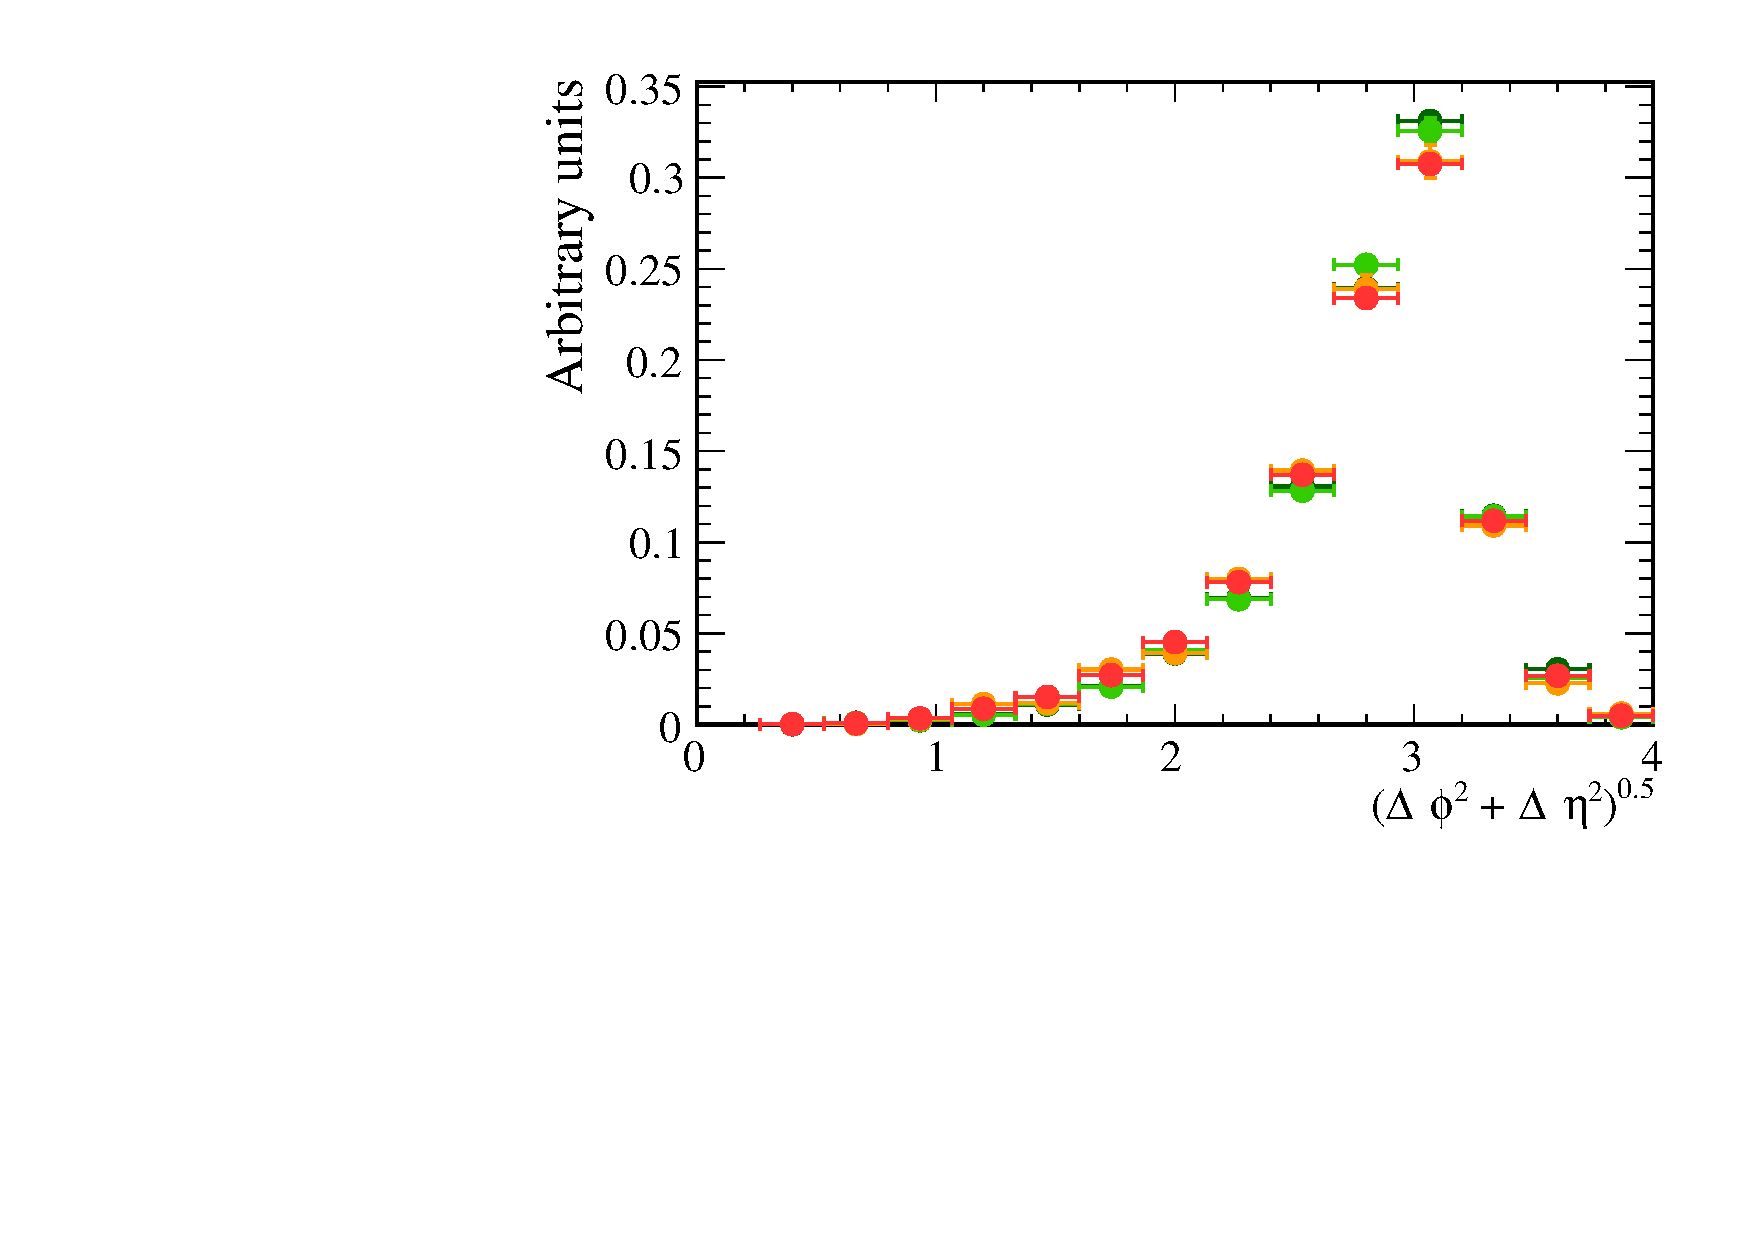
\includegraphics[width=\textwidth]{./Figs/Appendix1/bkgnf_DeltaR.pdf}
     %   \caption{ }
     %   \label{fig:BDTsig}
    \end{subfigure}
    ~ %add desired spacing between images, e. g. ~, \quad, \qquad, \hfill etc. 
      %(or a blank line to force the subfigure onto a new line)
    \begin{subfigure}[b]{0.48\textwidth}
       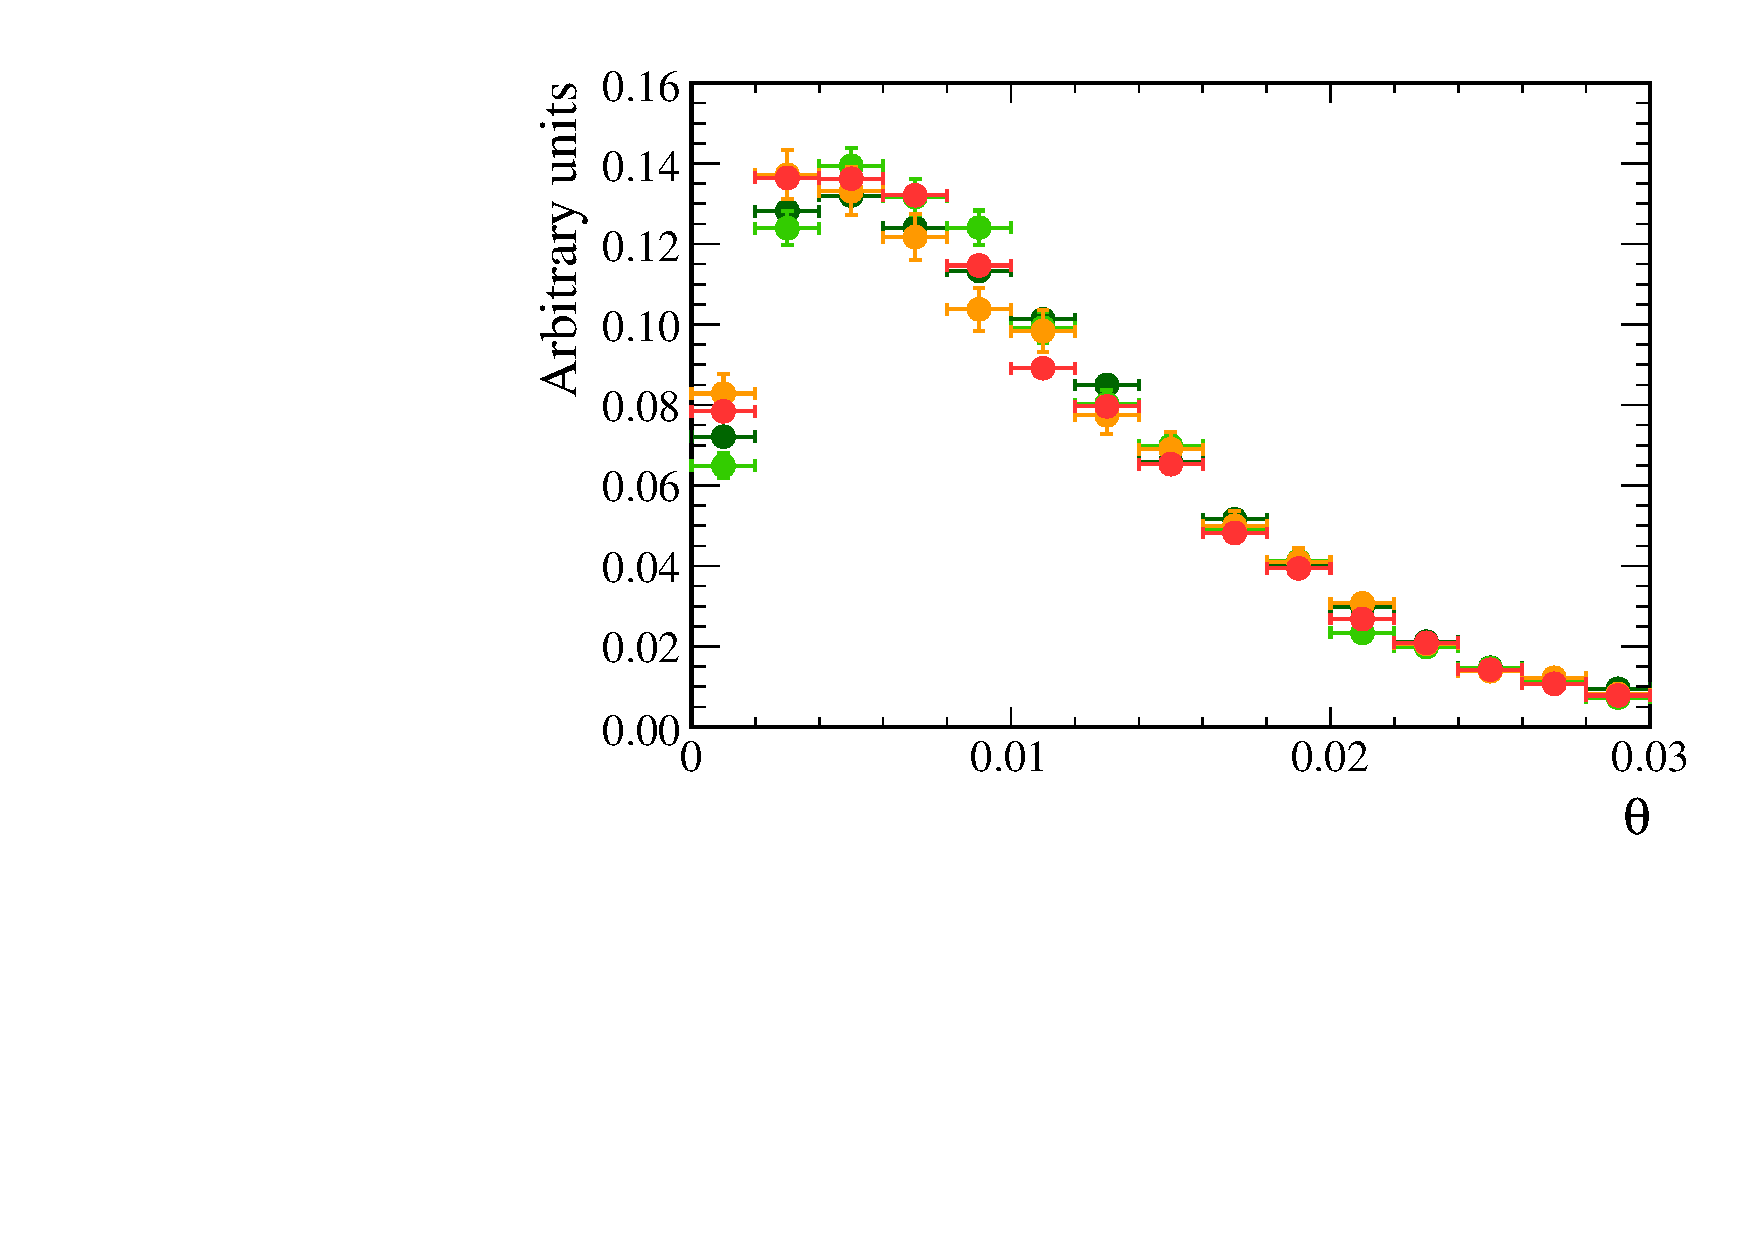
\includegraphics[width=\textwidth]{./Figs/Appendix1/bkgnd_DIRA.pdf}
    %    \caption{ }
    %    \label{fig:BDTbkg}
    \end{subfigure}



 \begin{subfigure}[b]{0.48\textwidth}
        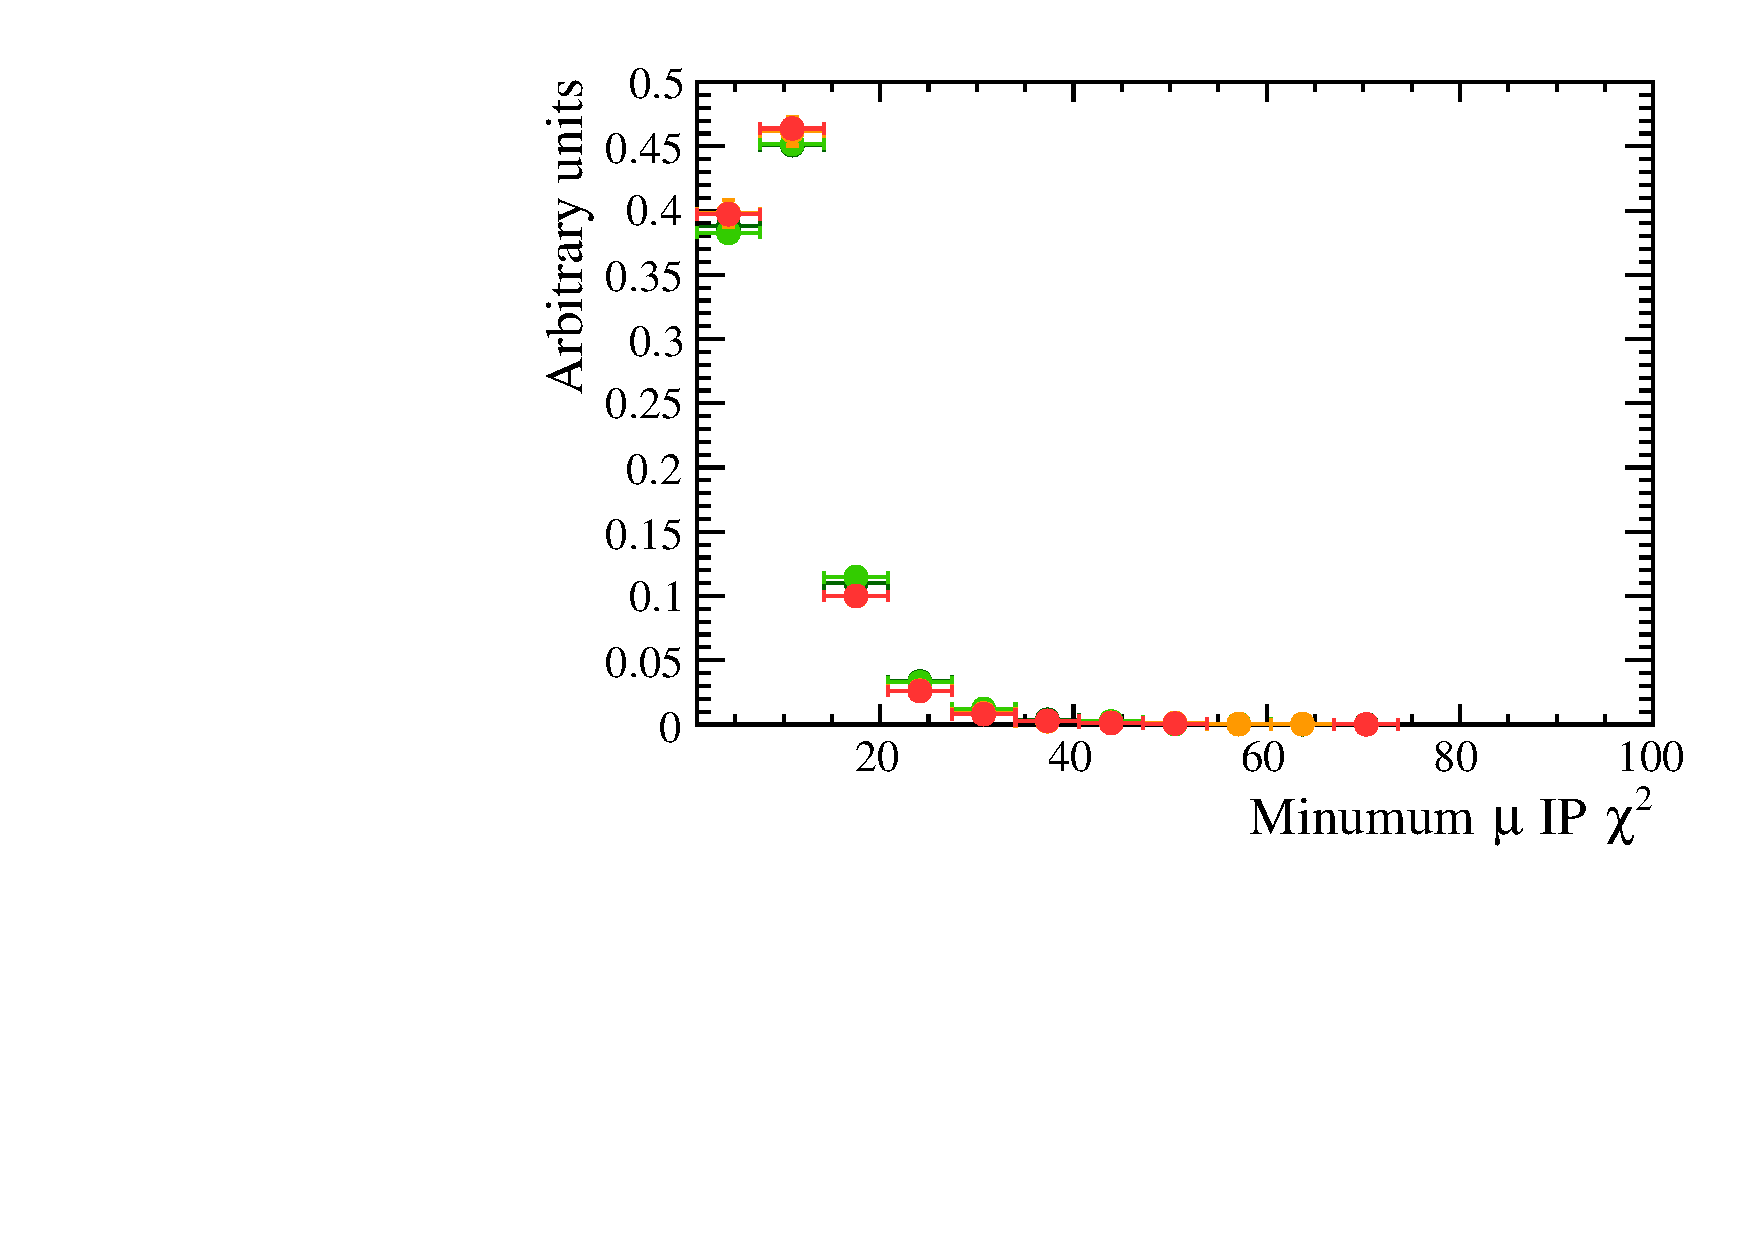
\includegraphics[width=\textwidth]{./Figs/Appendix1/bkgnd_muIPS.pdf}
      %  \caption{ }
      %  \label{fig:BDTsig}
    \end{subfigure}
    ~ %add desired spacing between images, e. g. ~, \quad, \qquad, \hfill etc. 
      %(or a blank line to force the subfigure onto a new line)
    \begin{subfigure}[b]{0.48\textwidth}
       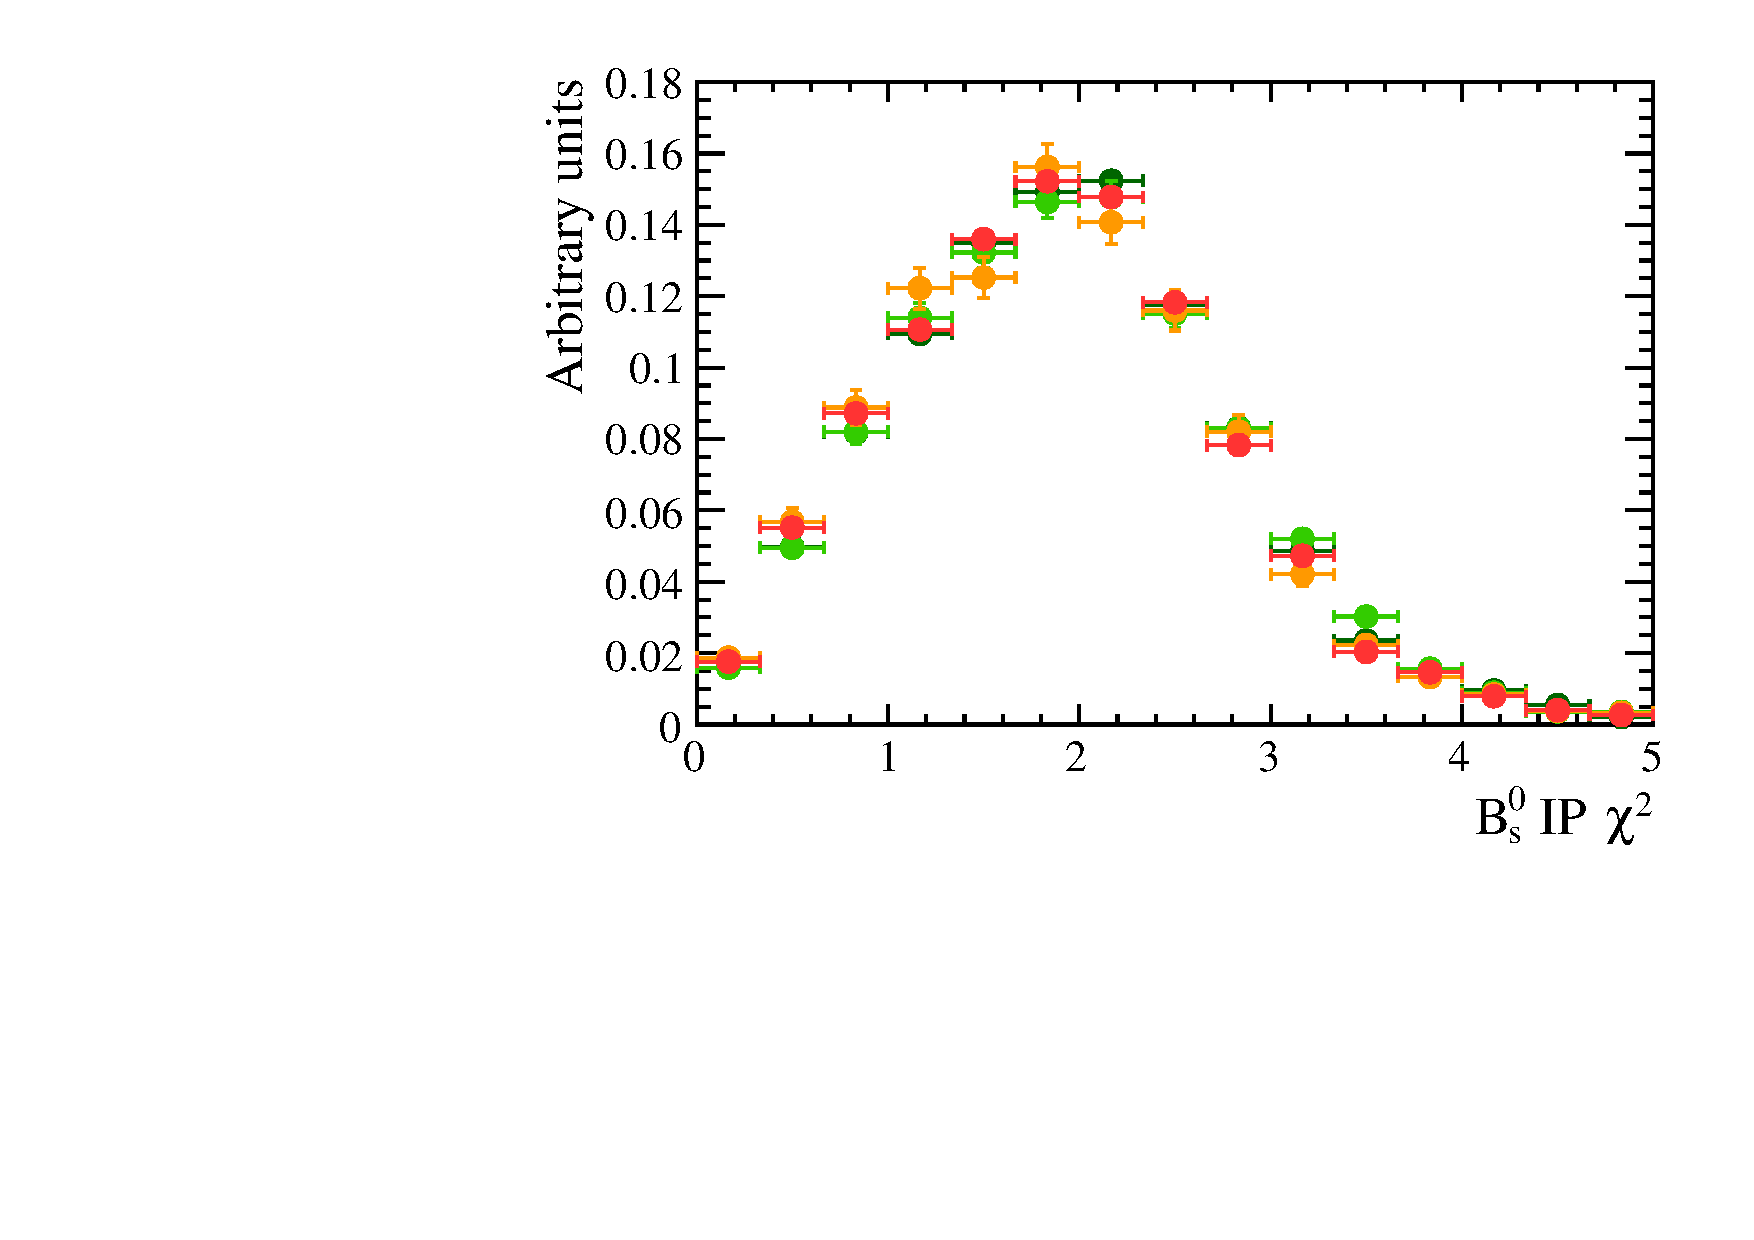
\includegraphics[width=\textwidth]{./Figs/Appendix1/bkgnd_IPS.pdf}
       % \caption{ }
       % \label{fig:BDTbkg}
    \end{subfigure}





 \begin{subfigure}[b]{0.48\textwidth}
        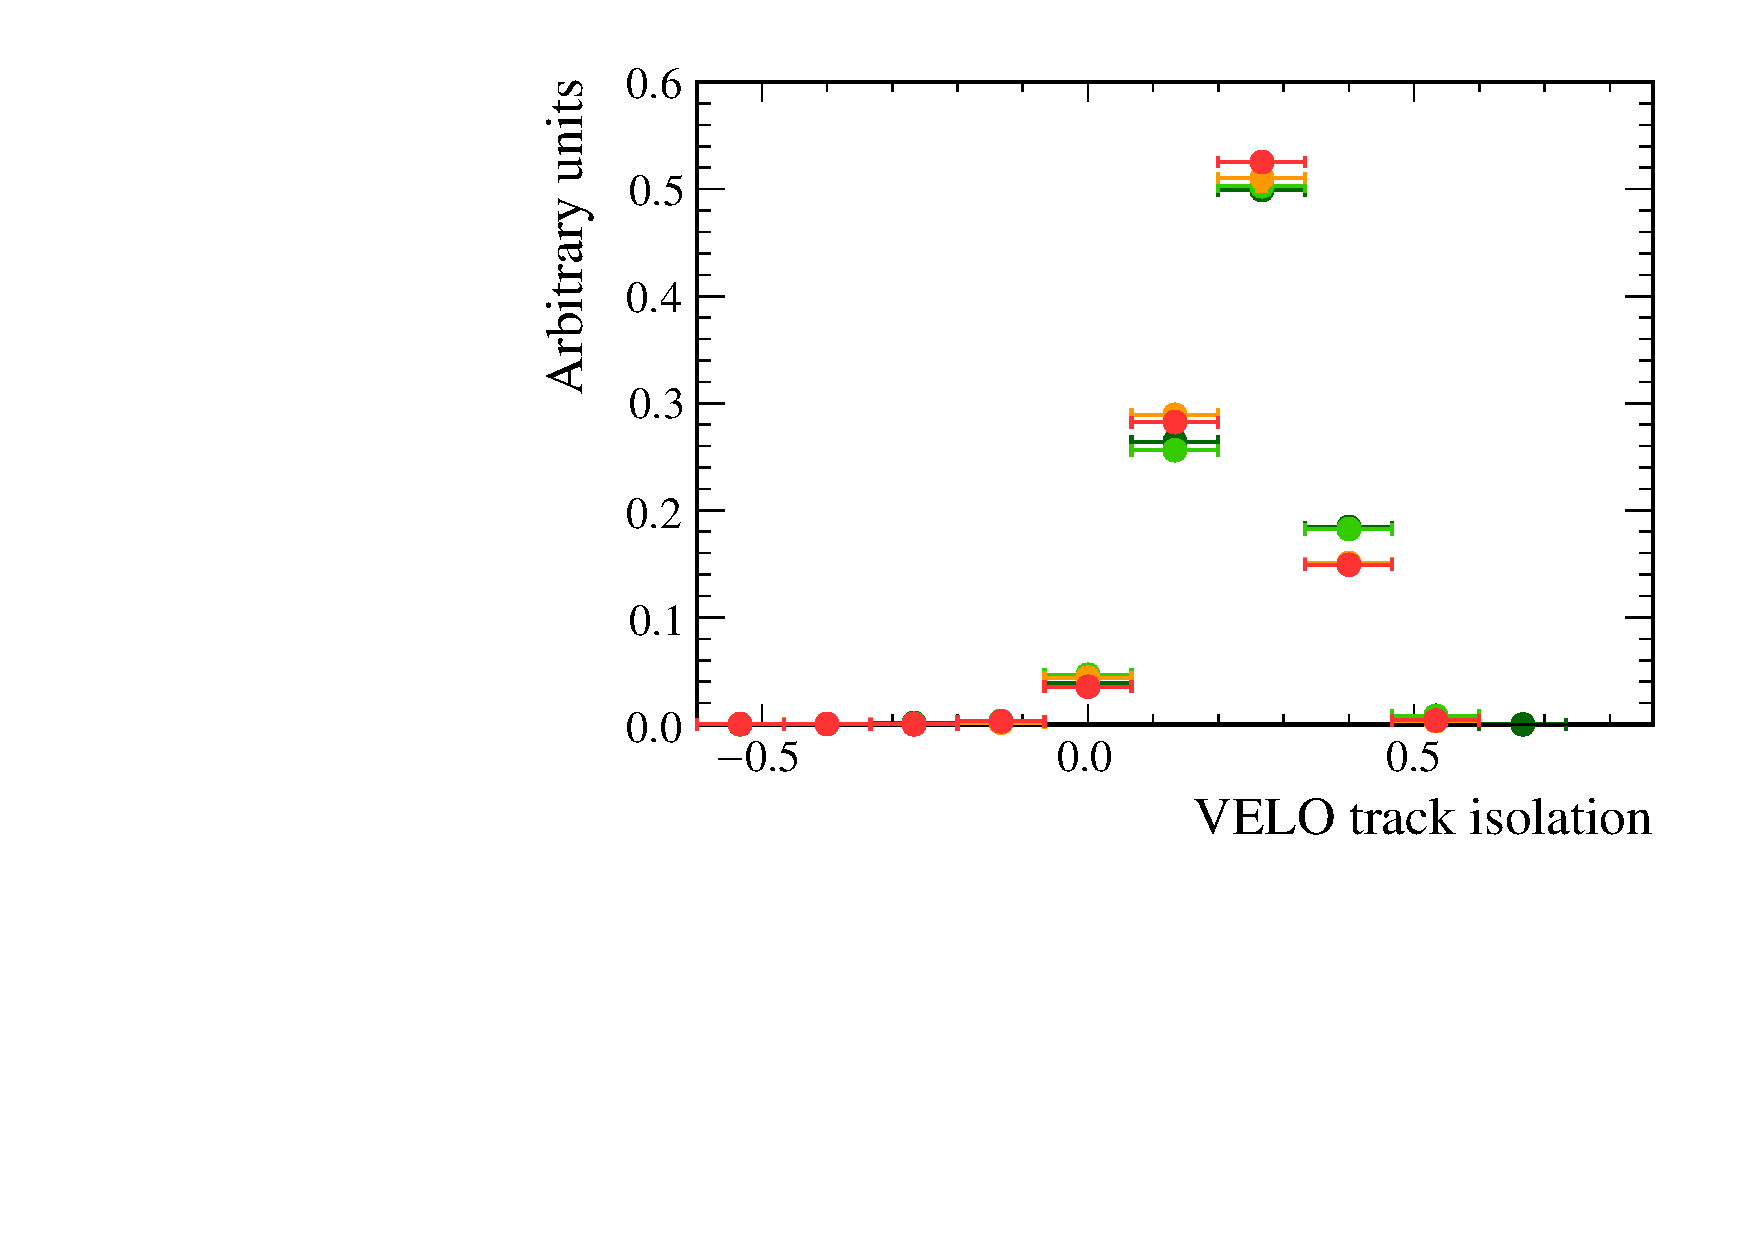
\includegraphics[width=\textwidth]{./Figs/Appendix1/bkgnd_iso_velo.pdf}
        %\caption{ }
        %\label{fig:BDTsig}
    \end{subfigure}
    ~ %add desired spacing between images, e. g. ~, \quad, \qquad, \hfill etc. 
      %(or a blank line to force the subfigure onto a new line)
    \begin{subfigure}[b]{0.48\textwidth}
       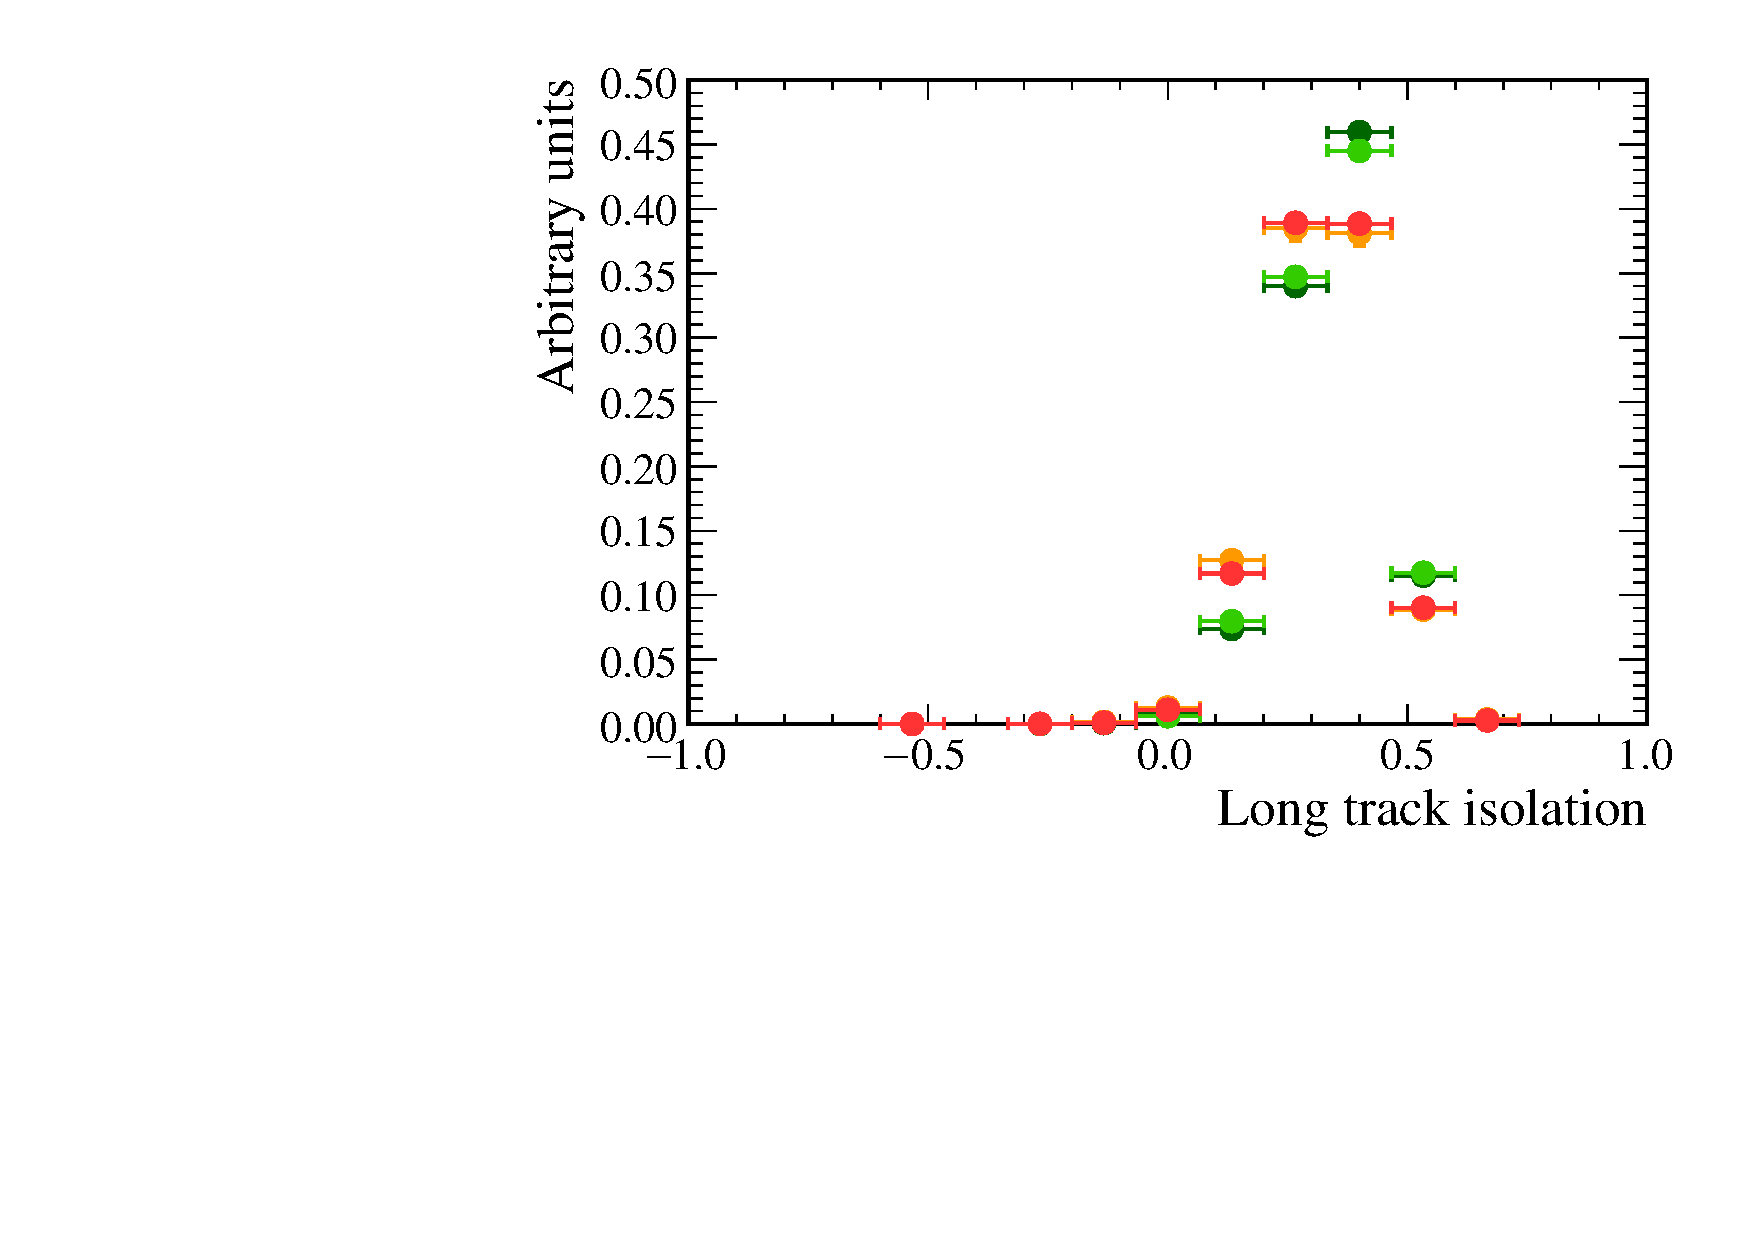
\includegraphics[width=\textwidth]{./Figs/Appendix1/bkgnd_long_iso.pdf}
        %\caption{ }
        %\label{fig:BDTbkg}
    \end{subfigure}




 \begin{subfigure}[b]{0.48\textwidth}
        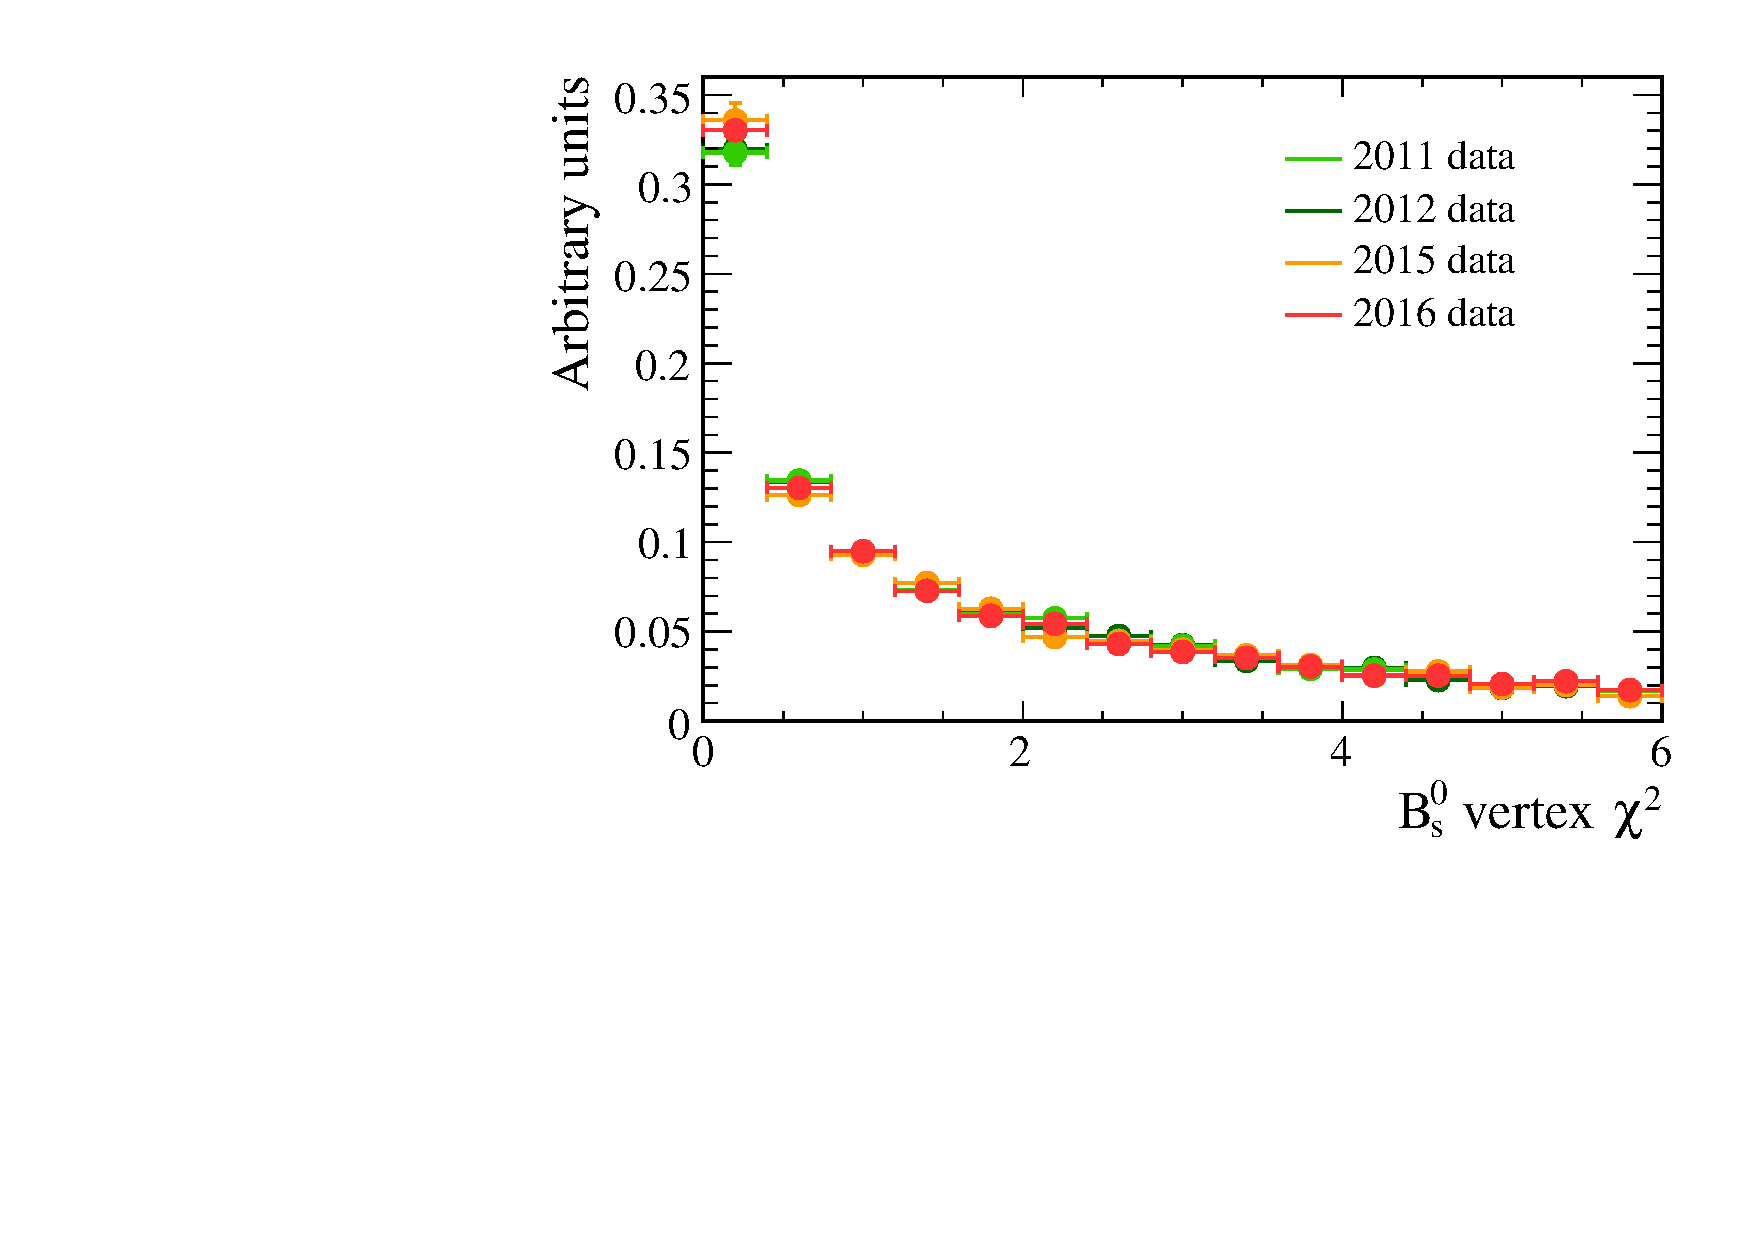
\includegraphics[width=\textwidth]{./Figs/Appendix1/bkgnd_vertex.pdf}
        \caption{ }
        \label{fig:BDTsig}
    \end{subfigure}
    ~ %add desired spacing between images, e. g. ~, \quad, \qquad, \hfill etc. 
      %(or a blank line to force the subfigure onto a new line)
 



    \caption{Background distributions for input variables from \bbbarmumux decays in 2011, 2012, 2015 and 2016 data with $m_{\mu \mu} > 5447$ \mevcc and 2012 simulated \bbbarmumux decays.}
    \label{fig:signalvars}
\end{figure}
